
\chapter{Introduction}


Manipulating the formation of a condensed phase is a critical part of both nature and technology. From molluscs controlling crystal formation~\cite{de-yoreo:03}, to molecular glasses to increasing the solubility of drugs~\cite{hancock:00}, to plastics\tocite, silicon in photovoltaic cells\tocite, and many other materials that we rely on every day. As the devices we use become smaller the need to understand the processes that form them becomes more important. A complete theory of glass formation is still elusive and our ability to control crystal formation is far from what is available to nature. To better understand the formation of the solid phase, we need an understanding of the molecular rearrangements that take place as we move from a molecular liquid, through a supercooled liquid to either a glass or molecular crystal.

\section{Molecular Crystals}

It might be expected the diversity in molecular shape will correspond to a diversity in molecular crystal structure. This is not the case, \SI{75}{\percent} of molecules occupy only five space groups~\cite{brock:94}. These space groups are a series of rotations, reflections, improper rotations, screw axes and glide planes that completely describe the unit cell of a crystal. There are 219 space groups in three dimensional space (230 including chiral copies) many of which are the basis of metallic crystal structures\tocite.

It has been proposed that the small distribution of space groups for molecular crystals is a result of how they pack space\tocite. One method of simulating crystal structures is assuming that atoms are hard spheres and finding the arrangement occupying the largest volume of space~\cite{kitaigorodskii:73}, also known as the \emph{packing fraction}. The simplest example of this is packing spheres, to which Kepler proposed the hexagonal closed packed structure~\figref{} in 1611\cite{kepler:1611}. However this is not a simple problem it has taken over 400 years to prove the hexagonal close packed structure gives the largest packing fraction~\cite{hales:05,hales:14}, requiring computers to check every possible configuration in space. More complicated systems are nigh impossible to prove. Fortunately finding a close packed structure is far simpler.

There are a number of computational tools used to find good approximations of closest packed structures\tocite. One of the simplifications that is made is to work in two dimensional space. This significantly simplifies the problem, now dealing with only 17 \emph{wallpaper groups}\figref{}. There have been a number of studies on the packing of convex shapes, however when dealing with a molecule there is going to be some degree of concavity~\figref{}. There has been less attention on concave shapes, however those that do show the p2 and the p2gg wallpaper groups make up nearly \SI{95}{\percent} of two dimensional molecular crystals~\tocite. \textcite{torquato:12} propose that concave particles without central symmetry will pair with the pair forming an inversion center; the p2 and p2gg wallpaper groups are the only ones that have this type of inversion center. 

The periodic and ordered structure that comes from the symmetry of the space group is also responsible for a number of properties of the crystal phase. These include mechanical properties such as hardness~\tocite or brittleness~\tocite, electrical properties\tocite, magnetic properties\tocite, even colour\tocite. For some applications the solid form is necessary however the crystal has unfavourable properties. An example of this is in drug design, a drug administered in tablet form needs to be solid, however it also needs to be soluble\tocite. Or in fiber optics where the fiber needs to be solid but also needs to be flexible\tocite. These applications can benefit from an amorphous solid, also known as a glass.

\section{Molecular Glasses}

The structure of a glass is indistinguishable from that of a liquid~\figref{}. Despite the liquid like structure the glassy phase is most definitely solid~\tocite, contrary to urban legends~\tocite. Much of the misunderstanding of the glassy phase is related to the lack of a first order phase transition~\tocite. None of the thermodynamic properties change upon transition, instead the \emph{glass transition temperature} (\si{\Tg}\tofix{$T_g$ definition}) is defined as the temperature at which the viscosity reaches \SI{e13}{\poise}, a somewhat arbitrary value. However as we approach the \si{\Tg} from the liquid there is a dramatic increase in the viscosity~\figref{}, especially for \emph{fragile} liquids.

Glass formers are characterised by their behaviour near \si{\Tg}. Liquids that adhere to a purely Arrhenius temperature dependence are considered \emph{strong} glass formers, the typical example being silica (\ce{SiO2}). Liquids with super-Arrhenius behaviour are considered \emph{fragile}, \emph{o}-terphenyl being the canonical example. A system that displays Arrhenius temperature dependence,
\begin{equation}
    k = A \e^{-E_a/(RT)}
\end{equation}
has an energy barrier that requires an activation energy ($E_a$) to surmount. This activation energy remains constant throughout the temperature range. Fragile liquids however have an activation energy that depends on the temperature\tocite, characterised by large increases in viscosity over a small temperature range as \si{\Tg} is approached. The temperature dependence of the viscosity in fragile liquids indicates that the glass transition temperature is more than just an arbitrary value, rather; the glass transition is an inherent characteristic of a material.

Developing a theoretical understanding of a material requires a model system, something simple enough to model easily, yet close enough to a real world example. A defining feature of fragile glass formers~\tabref{} is the prominence of molecular liquids, making simple molecular liquids a good choice for a model system.


\begin{figure}
    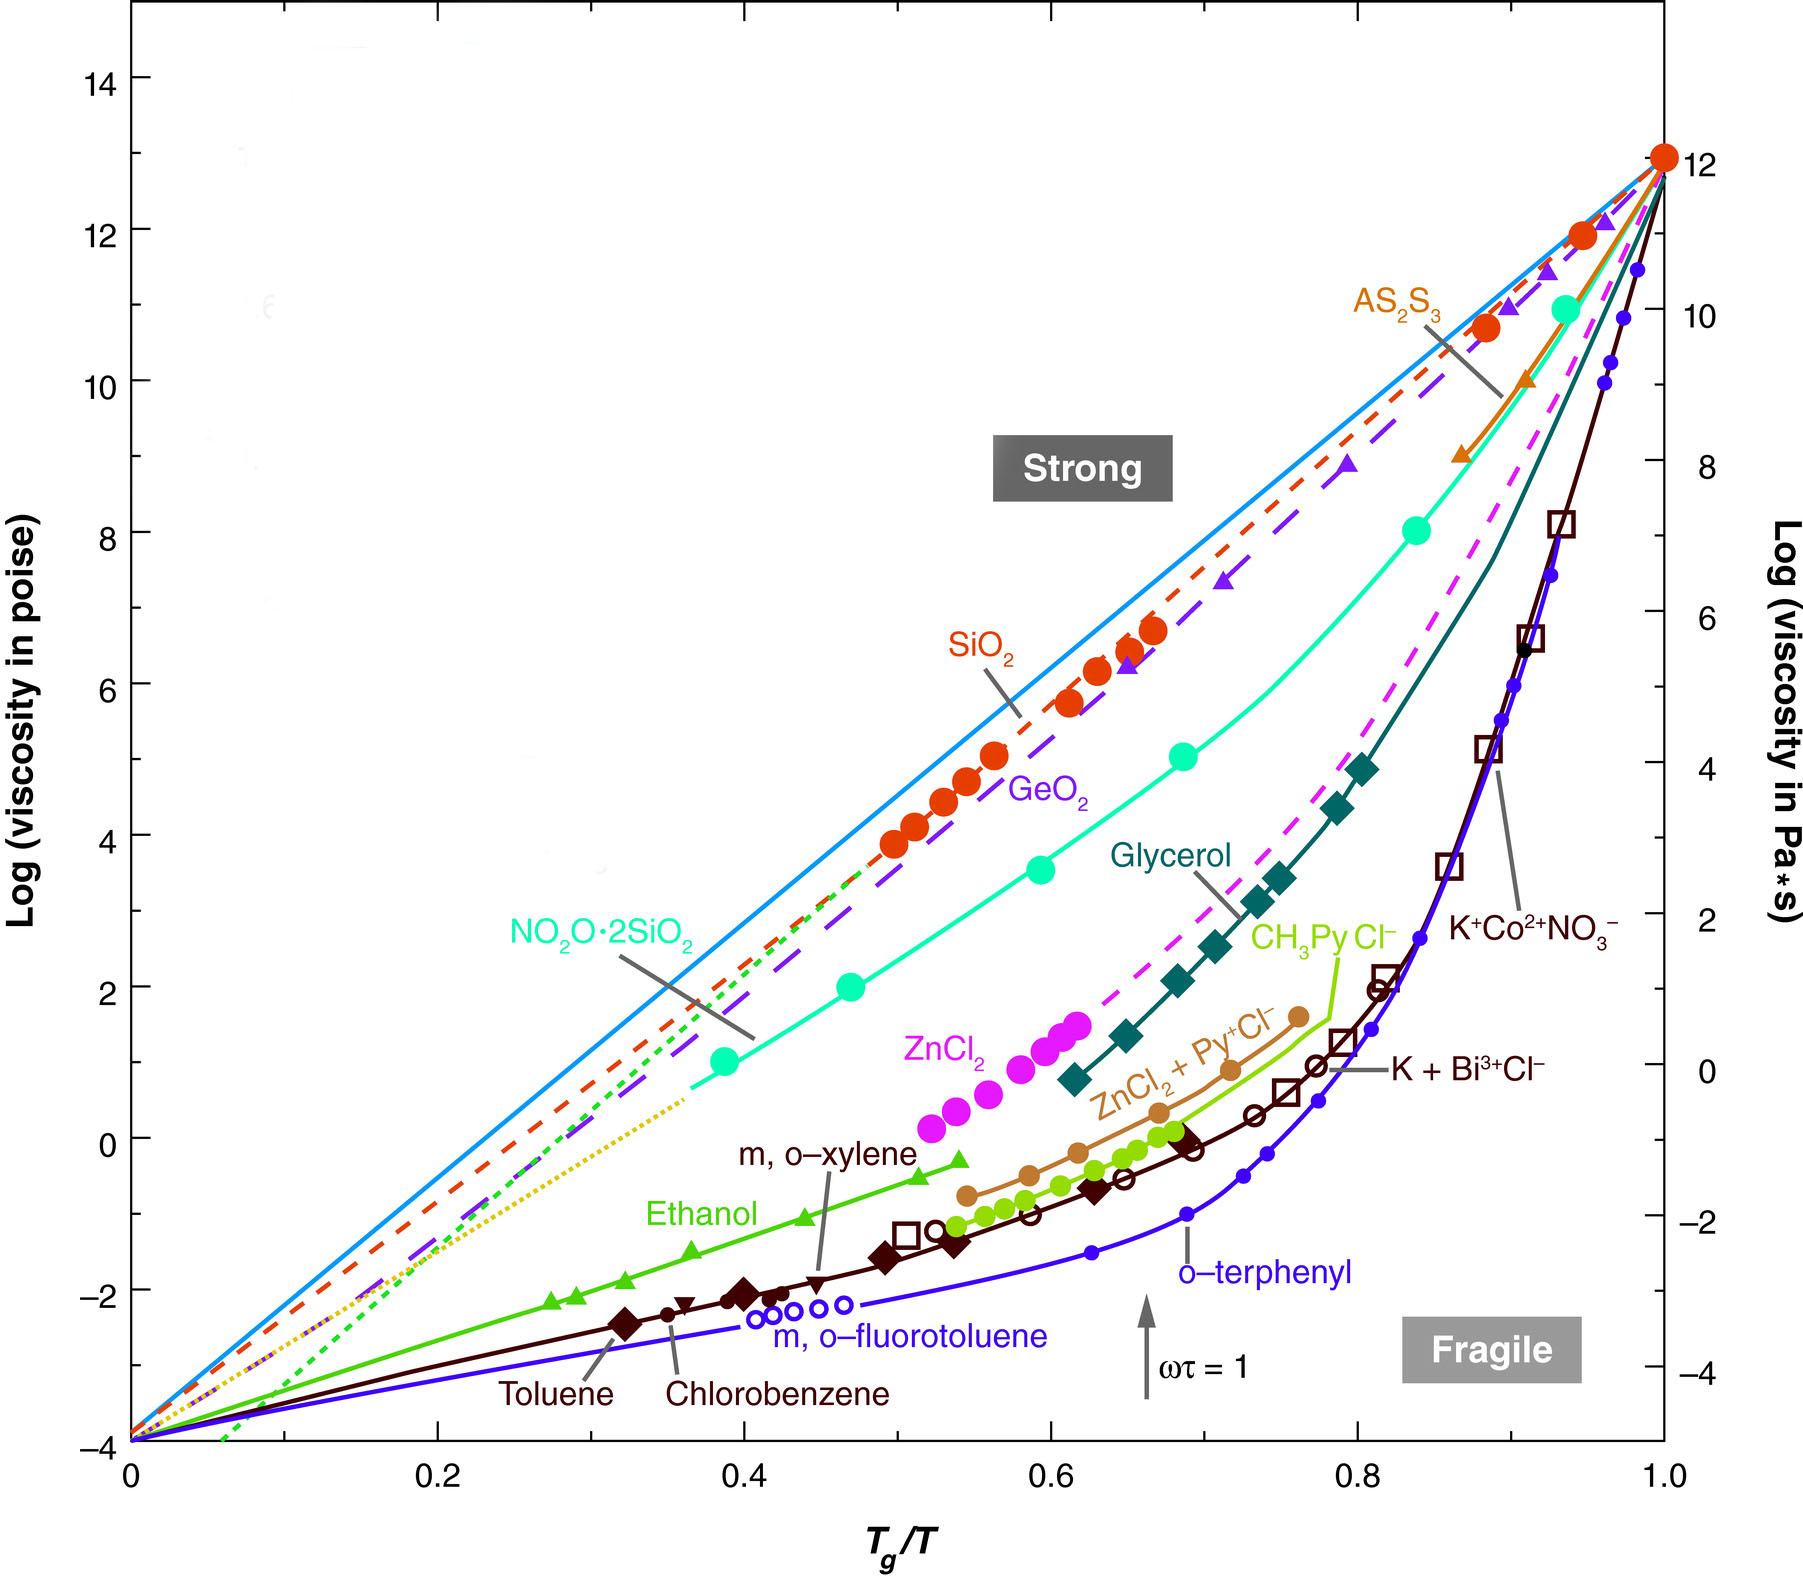
\includegraphics[width=\textwidth]{angell}
    \caption{Angell plot (from \textcite{lubchenko:07}, used with permissioni Annual reviews)}
    \label{fig:entropy}
\end{figure}

\section{Liquids}

\section{Project Goals}

The goal of my project is to explore fundamental features of molecular shape; asymmetry and concavity, influence the properties of the various condensed phases; liquid, crystal, glass and supercooled-liquid. This requires the characterisation of a new set of molecular models for computer simulation. I will be addressing how the molecular orientation and translational motion couple during crystal growth, how the degree of concavity in the molecular shape determines the dynamics of rotations and translations in the low temperature liquid phase and, to find stable structures that determine the properties of crystals and glasses and how these structures are influenced by molecular shape.

